\documentclass[10pt,a4paper]{article}
\usepackage[margin=0.62in,top=0.58in,bottom=0.60in]{geometry}
\usepackage[T1]{fontenc}
\usepackage[utf8]{inputenc}
\usepackage{lmodern,microtype}
\usepackage{amsmath,amssymb}
\usepackage{booktabs,tabularx,array}
\usepackage{graphicx}
\usepackage[table]{xcolor}
\usepackage[font=small,labelfont=bf]{caption}
\usepackage{enumitem}
\usepackage[hidelinks]{hyperref}
\usepackage{fancyhdr,titlesec,float}

\definecolor{ink}{HTML}{1F2937}
\definecolor{accent}{HTML}{185A88}
\definecolor{muted}{HTML}{596878}
\hypersetup{colorlinks=true,linkcolor=accent,urlcolor=accent}
\titleformat{\section}{\large\bfseries\color{ink}}{\thesection}{0.55em}{}
\titleformat{\subsection}{\normalsize\bfseries\color{ink}}{\thesubsection}{0.5em}{}
\titlespacing*{\section}{0pt}{0.65em}{0.25em}
\titlespacing*{\subsection}{0pt}{0.45em}{0.15em}
\setlength{\parindent}{0pt}
\setlength{\parskip}{0.16em}
\setlist[itemize]{leftmargin=1.3em,itemsep=0pt,topsep=1pt}
\setlist[enumerate]{leftmargin=1.4em,itemsep=0pt,topsep=1pt}
\captionsetup{skip=3pt}
\pagestyle{fancy}\fancyhf{}
\fancyhead[L]{\footnotesize\color{muted} Long-Horizon State Tracking with Compact Mamba}
\fancyhead[R]{\footnotesize\color{muted} Research Report}
\fancyfoot[C]{\footnotesize\thepage}
\renewcommand{\headrulewidth}{0.25pt}
\newcommand{\SET}{\texttt{SET}}
\newcommand{\QUERY}{\texttt{QUERY}}
\newcommand{\NOOP}{\texttt{NOOP}}
\newcommand{\UNSET}{\texttt{UNSET}}
\newcolumntype{Y}{>{\raggedright\arraybackslash}X}
\newcolumntype{C}{>{\centering\arraybackslash}X}
\renewcommand{\arraystretch}{1.10}
\definecolor{softblue}{HTML}{EEF5F9}
\definecolor{softgreen}{HTML}{EAF6EE}
\definecolor{softamber}{HTML}{FFF5DF}
\definecolor{softred}{HTML}{FBEDEE}

\title{\vspace{-1.8em}\textbf{Long-Horizon State Tracking with Compact Mamba}\\[-0.05em]
\large Retention, Interference, and Controlled Negative Architecture Results}
\author{HackerRank Deep Learning Research Engineer Assignment\\
\small Primary architecture comparison: seed 42; supplementary diagnostics: seeds 42--46}
\date{November 2026}

\begin{document}
\maketitle
\vspace{-1.45em}
\fontsize{9.4pt}{10.9pt}\selectfont

\begin{abstract}\small
We study whether a compact selective state-space model can maintain eight logical key--value registers when evaluation sequences are four times longer than those used for training. The one-layer Mamba baseline reaches 69.64\% aggregate query accuracy at length 512, but balanced retrieval falls from 84.38\% after 10 passive steps to chance after 500. Unrelated-key SET events are more damaging than matched NOOP and QUERY controls, yet key-conditioned write routing does not beat a parameter-matched tied control. Mechanistic interventions instead implicate recurrent retention: after the width-four convolution completes its three-step response, forcing later NOOP recurrence to identity restores approximately 97\% accuracy through delay 128. We then train a fast/slow state decomposition and an identity-default slow-memory gate. Finally, H8 separates slow-memory erasure from writing and compares it with an exactly parameter-matched tied-gate model. Decoupling is falsified at seed 42: its delay-511 accuracy is 31.25\%, versus 40.23\% for the tied gate and 39.45\% for constrained fast/slow Mamba. The tied gate simultaneously achieves 100\% overwrite accuracy through 32 post-overwrite steps and zero stale-value errors. These results support event-selective near-identity recurrence, but not unconstrained independent erase/write decisions.
\end{abstract}

\section{Introduction}
Selective state-space models combine structured recurrent dynamics with input-dependent selection \cite{s4,mamba}. The task here appears simple at the symbolic level: \SET{} replaces the value associated with one of eight keys, \QUERY{} requests the most recent value, and \NOOP{} leaves the correct dictionary unchanged. It is nevertheless a useful stress test because success requires three behaviors that need not coincide in a learned continuous state: preserve an assignment through long passive intervals, overwrite it quickly when the same key changes, and update other keys without corrupting it. The central research question is therefore not only whether accuracy decreases at length 512, but \emph{which operation fails and why}.

Our investigation follows a sequence of discriminating experiments. We first reproduce the assignment baseline and separate aggregate sequence-length accuracy from controlled SET-to-QUERY delay. We then introduce unrelated SET and QUERY distractors to distinguish cross-key writes from generic active-token processing. The resulting interference motivates key-conditioned write routing and a parameter-matched control. When this proposal fails, frozen interventions isolate recurrent decay from incoming writes, a convolution-aware identity intervention tests whether passive state evolution is causal, and independent probes localize accessible information. Supplementary adaptive-kernel experiments test local context control. The final H7/H8 sequence moves from diagnosis to trained recurrence: constrained fast/slow modes, an identity-default slow update, and then separate erase/write gates with a tied-gate control. At each stage we distinguish measured behavior, interpretation, and falsification.

\paragraph{Contributions.} The study provides (i) a reproducible compact-Mamba baseline on the mandated fixed splits; (ii) multi-seed evidence for long-delay degradation and cross-key interference; (iii) controlled negative results for key routing, adaptive convolution, and independently gated erase/write memory; (iv) causal evidence that late passive transitions drive much of the forgetting; (v) probe evidence that preservation and retrieval can become misaligned; and (vi) a trained tied-gate control that combines long retention with clean overwrite behavior in the seed-42 pilot.

\section{Task and Model}
Each input timestep is one of 41 logical tokens: one \NOOP, 32 key--value-specific \SET{} tokens, or eight key-specific \QUERY{} tokens. The target vocabulary is \(\{\UNSET,1,2,3,4\}\). Targets at SET and NOOP positions are masked with \texttt{-100}; consequently, the cross-entropy objective and all reported task accuracies use QUERY positions only. The answer is never included in the input. A deterministic dictionary simulator supplies both the labels and a 100\% exact oracle, while the Always-UNSET predictor provides a length-dependent constant baseline.
\begin{table}[!htbp]
\centering\small
\caption{Task and implementation invariants.}
\begin{tabularx}{\linewidth}{p{0.20\linewidth}p{0.27\linewidth}Y}
\toprule
Component & Fixed setting & Why it matters \\
\midrule
Events & 32 \SET, 8 \QUERY, 1 \NOOP{} token & Eight independent keys; four possible assigned values \\
Prediction & \(\{\UNSET,1,2,3,4\}\) & QUERY contains the key but never the target value \\
Backbone & 1 layer, \(d_{\rm model}=32\), \(d_{\rm state}=8\), expand 2 & Compact 10,149-parameter baseline \\
Local mixing & Causal depthwise convolution, width 4 & A SET response can continue for three later steps \\
SSM memory & \(64\times8=512\) recurrent coordinates & All eight logical keys share one recurrent state \\
Objective & Query-only CE; non-queries masked with \texttt{-100} & Prevents non-query supervision and target leakage \\
Verification & 34 automated tests, all passing & Oracle, overwrite, UNSET, masking, gradients, and causality \\
\bottomrule
\end{tabularx}
\end{table}

For convolution-processed input \(u_t\), the readable selective scan is
\begin{align}
h_t &= \exp(\Delta_tA)\odot h_{t-1}+\Delta_tB_tu_t,\\
r_t &= C_th_t+D\odot u_t, \qquad A=-\exp(A_{\log})<0.
\end{align}
The event ID is embedded into 32 dimensions, projected to the 64-dimensional inner width, and passed through the causal depthwise convolution and SiLU nonlinearity to obtain \(u_t\). The input-dependent step size \(\Delta_t\) controls how strongly the state both decays and changes; \(B_t\) determines how the current event is written into the eight state modes; and \(C_t\) contracts those modes back into a per-channel output. The direct \(D\odot u_t\) path, output gate, projection, residual connection, and final normalization produce a 32-dimensional feature that is classified by \(\mathrm{Linear}(32,5)\). Because all eight logical keys share these recurrent coordinates and projections, good overwrite behavior does not guarantee either long retention or isolation from unrelated updates.

The implementation preserves four invariants from the upstream model: strictly causal convolution, left-to-right selective scan, the fixed assignment dimensions, and query-only supervision. Changes are injected through optional per-position write or decay multipliers inside the readable scan; when absent, the baseline path is numerically unchanged. Tests cover token/target construction, oracle overwrite semantics, UNSET queries, masking, tensor shape, finite gradients, causality, checkpoint continuation, and the interfaces introduced by the experimental variants.
\begin{center}
\small\fbox{\parbox{0.92\linewidth}{\textbf{Mechanistic decomposition:} repeated \(\exp(\Delta_tA)\) controls retention; \(\Delta_tB_tu_t\) introduces new writes; \(C_th_t+D\odot u_t\) determines what is exposed to the downstream classifier.}}
\end{center}

\section{Hypotheses and Protocol}
The experimental design deliberately moves from behavior to mechanism. H1 removes overwrites and cross-key writes, leaving only elapsed passive transitions. H2 fixes elapsed delay and changes the type and density of intervening activity. Part B then tests whether key-specific control of the input-write term addresses H2. The later interventions are diagnostic perturbations of frozen models, not proposed benchmark replacements; their purpose is to decide which term deserves a trained architectural follow-up.
The predeclared decision rules are deliberately mechanism-specific. H1 is falsified if balanced long-delay retrieval does not decline; H2 if unrelated SETs are not worse than matched controls above the chance floor; key routing if it fails to exceed the tied control by 2 points; H4 if a convolution-aware identity intervention does not rescue retrieval; H5 if a matched long-horizon readout cannot exploit the modified features; adaptive convolution if token conditioning does not beat static mixing; and H8 if independent erase/write gates do not beat their parameter-matched tied control on delay-511 retention without increasing stale-value errors.

\addtocounter{table}{1}% preserve numbering of the full hypothesis table in the detailed record
\begin{table}[!htbp]
\centering\small
\caption{Matched training and evaluation protocol.}
\begin{tabularx}{\linewidth}{p{0.23\linewidth}Y p{0.28\linewidth}}
\toprule
Item & Setting & Control \\
\midrule
Train / validation & 4,000 / 500 sequences, lengths 32--128 & Same files for all architectures \\
Fixed tests & 500 each: ID-128, OOD-256/512, delay/overwrite-512 & Exact oracle and Always-UNSET baselines \\
Optimization & FP32 AdamW, LR \(10^{-3}\), batch 16 & 1,500 updates; checkpoint chosen on validation only \\
H1 & Balanced 8 keys \(\times\) 4 values; seeds 42--44 & Delays 10, 32, 64, 128, 256, 500 \\
H2 & 1,024 paired examples/condition; seeds 42--46 & NOOP and unrelated-QUERY active-token controls \\
Uncertainty & Paired/hierarchical bootstrap where paired & Seed-level H1 intervals labeled \(n=3\) \\
\bottomrule
\end{tabularx}
\end{table}

All architecture comparisons use identical generated training data, data order, optimizer settings, and update counts. The initial 300-update baseline follows the requested starting budget but remains near the trivial baselines, so it is extended to 1,500 updates; this deviation is disclosed rather than selecting a favorable stress result. Fixed test labels are never used for checkpoint selection. H1 intervals summarize variation over three independently trained models. H2 and the causal NOOP experiment use five models. Paired bootstrap intervals reuse the same examples across contrasted conditions, while architecture results based only on seed 42 are interpreted using a predeclared two-percentage-point practical threshold rather than sub-point rankings.

\section{Baseline Results and Failure Diagnosis}
\subsection{Aggregate learning and length generalization}
Table 4 reports accuracy over \emph{every} QUERY in each fixed split. This is appropriate for the assignment-wide benchmark, but it weights the many short and moderate dependencies much more heavily than the single designed final probe in each stress sequence. The controlled analyses below therefore report both aggregate accuracy and final-query behavior.
\begin{table}[!htbp]
\centering\small
\caption{All-query accuracy (\%) on the fixed assignment splits. The exact dictionary oracle is 100\% on every split.}
\begin{tabular}{lrrrr}
\toprule
Split & Length & 300 updates & 1,500 updates & Always UNSET\\
\midrule
ID & 128 & 25.67 & \textbf{75.05} & 23.28\\
OOD & 256 & 14.81 & \textbf{71.23} & 11.28\\
OOD & 512 & 10.45 & \textbf{69.64} & 5.97\\
Delay stress & 512 & 8.64 & \textbf{69.59} & 4.21\\
Overwrite stress & 512 & 8.86 & \textbf{69.67} & 4.28\\
\bottomrule
\end{tabular}
\end{table}

The 300-update model has not yet learned robust state tracking: at ID-128 it reaches 25.67\%, only 2.39 points above Always UNSET, and its stress accuracy is below 9\%. Extending the same configuration to 1,500 updates raises ID-128 accuracy to 75.05\% and retains 69.64\% at OOD-512. The modest 5.41-point drop from ID-128 to OOD-512 suggests useful length generalization in aggregate. It does \emph{not}, however, establish 512-step memory: ordinary long sequences contain many recent SETs, so a model can answer most queries without preserving a value across the full sequence.

\subsection{H1: isolating passive retention}
For each model seed and delay, the H1 probe balances all \(8\times4\) key--value combinations. A 32-token randomized burn-in is followed by one SET of the tracked key, exactly \(d\) NOOPs, and a final QUERY of that key. No overwrite or unrelated update occurs between SET and QUERY. Thus, changing \(d\) changes only the number of passive recurrent transitions.

\begin{table}[!htbp]
\centering\small
\caption{H1 balanced retrieval by SET-to-QUERY delay (mean across seeds 42--44).}
\resizebox{\linewidth}{!}{%
\begin{tabular}{lrrrrrr}
\toprule
Delay & 10 & 32 & 64 & 128 & 256 & 500 \\
\midrule
Accuracy (\%) & \cellcolor{softgreen}84.38 & 64.58 & 45.83 & 28.13 & 23.96 & \cellcolor{softred}25.00 \\
Drop from delay 10 (pp) & 0 & 19.80 & 38.55 & 56.25 & 60.42 & 59.38 \\
\bottomrule
\end{tabular}
}
\end{table}
The delay-10 to delay-128 drop is 56.25 pp (95\% seed-level CI 40.72--71.78); delay 500 reaches four-value chance even though aggregate OOD-512 accuracy is 69.64\%. H1 is therefore supported: the model's strong aggregate score is compatible with catastrophic failure on a dependency that actually spans the evaluation sequence. The wide early confidence intervals reflect only three training seeds, but all seeds approach chance at the longest delay.

\begin{figure}[!htbp]
\centering
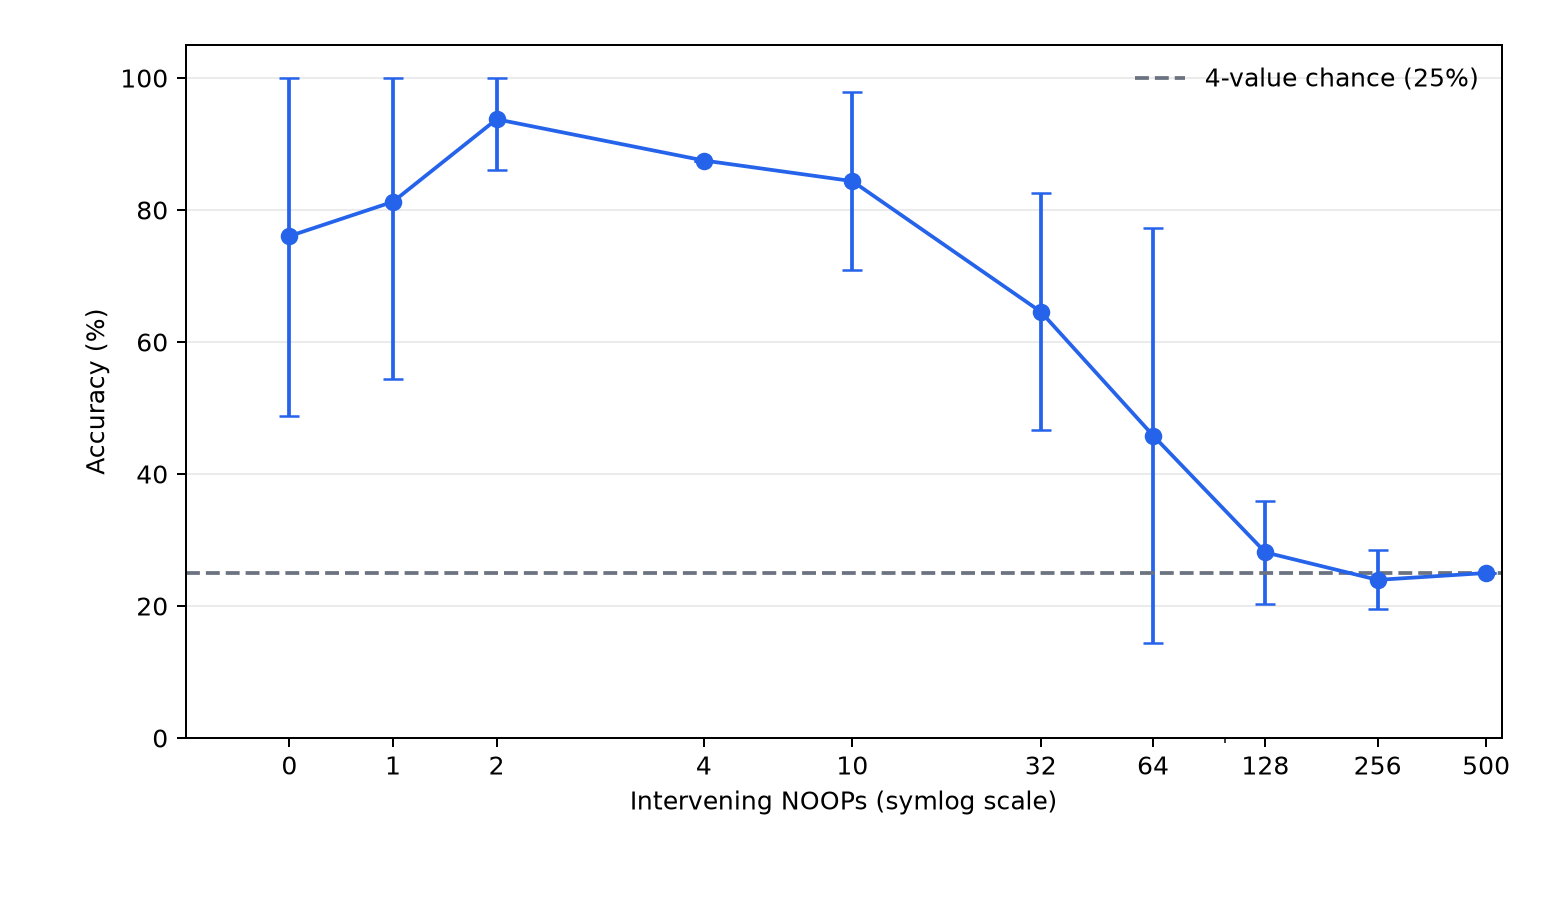
\includegraphics[width=0.78\linewidth]{figures/retention_by_delay.png}
\caption{Balanced retrieval degrades with intervening NOOPs across three training seeds. Error bars are seed-level 95\% intervals; wide early intervals reflect \(n=3\), while the approach to chance is consistent across seeds.}
\label{fig:h1}
\end{figure}

\subsection{H2: separating writes from generic activity}
H2 keeps the tracked SET-to-QUERY delay fixed and replaces a nested fraction of the intervening NOOP positions with events involving the other seven keys. The SET condition changes an unrelated key--value association; the QUERY condition uses the same positions and key identities but performs no logical write. Each condition contains 1,024 examples per model, balanced over tracked keys and values, and the same base example is reused across conditions. This pairing makes SET-minus-NOOP a total active-write effect and SET-minus-QUERY a more specific estimate of the additional cost of writing.

\begin{table}[!htbp]
\centering\small
\caption{H2 at 100\% distractor density (five seeds; accuracy in \%).}
\begin{tabular}{lrrrr}
\toprule
Condition / effect & Delay 10 & Delay 32 & Delay 64 & Delay 128 \\
\midrule
NOOP control & 93.16 & 82.23 & 54.16 & 29.47 \\
Unrelated QUERY & 92.52 & 60.72 & 27.77 & 20.23 \\
Unrelated SET & 78.67 & 31.74 & 21.80 & 21.21 \\
SET minus NOOP (pp) & -14.49 & \cellcolor{softred}-50.49 & -32.36 & -8.26 \\
SET minus QUERY (pp) & -13.85 & -28.98 & -5.98 & +0.98 \\
\bottomrule
\end{tabular}
\end{table}
At delays 10--64, unrelated SETs are materially worse than matched QUERYs, so cross-key writing contributes beyond generic active-token processing. At delay 32, for example, SET-minus-NOOP is \(-50.49\) points (95\% hierarchical-bootstrap CI \([-53.91,-46.93]\)) and SET-minus-QUERY is \(-28.98\) points (\([-37.97,-19.61]\)). The QUERY control also degrades strongly at delays 32 and 64, showing that the failure is not purely write collision. Delay 128 is floor-limited: the NOOP control is already near four-value chance, leaving little dynamic range for a mechanism-specific contrast. H2 is supported over the usable operating range, while the floor-limited comparison is treated as inconclusive rather than contradictory.

\section{Part B: Key-Conditioned Write Routing}
The H2 result suggests a natural architectural hypothesis: unrelated keys may interfere because their SET events write through overlapping inner channels. A key-conditioned router could encourage different logical keys to use different channel patterns. This is intentionally a narrow modification of the input-write pathway; it does not alter the state matrix, recurrent decay, convolution, query readout, or output head.

The proposed model learns \(R\in\mathbb R^{8\times64}\). A SET to key \(k\) uses \(g_k=\sigma(R_k)\) to gate only the input-write term:
\begin{equation}
h_t=\exp(\Delta_tA)\odot h_{t-1}+g_k\odot(\Delta_tB_tu_t).
\end{equation}
This adds 512 parameters (10,661 total, +5.0\%). Non-SET writes are unchanged. The decisive ablation retains the same \(8\times64\) parameter tensor and routing computation but averages its rows before use. It therefore matches parameter count and optimization opportunity while removing the only proposed mechanism---dependence on key identity. Both routed models initialize to gate value 0.95 and are trained for 1,500 updates on the same seed-42 examples and data order as the baseline. The hypothesis is falsified if key-conditioned routing fails to beat this tied control by the predeclared 2-point margin under dense cross-key interference.

\begin{table}[!htbp]
\centering\small
\caption{Matched 1,500-update models: all-query accuracy (\%).}
\begin{tabular}{lrrrrr}
\toprule
Model & ID-128 & OOD-256 & OOD-512 & Delay & Overwrite\\
\midrule
Baseline & 75.05 & 71.23 & 69.64 & 69.59 & \textbf{69.67}\\
Key-conditioned & \textbf{75.57} & \textbf{71.54} & \textbf{69.86} & \textbf{70.06} & 69.55\\
Tied routing & 75.50 & 71.42 & 69.75 & 69.96 & 69.50\\
\bottomrule
\end{tabular}
\end{table}

The routed models are slightly above baseline on four aggregate splits, but the key-conditioned and tied variants differ by at most 0.12 points. Since the tied model cannot isolate keys, these aggregate gains can be explained by additional global write rescaling or optimization capacity. The mechanism-specific dense-interference contrast provides the stronger test.

\begin{table}[!htbp]
\centering\small
\caption{Mechanism-specific routing evidence.}
\begin{tabularx}{\linewidth}{Y C C C C}
\toprule
Measure & Delay 10 & Delay 32 & Delay 64 & Delay 128 \\
\midrule
Key minus tied at 100\% SET density (pp) & +0.49 & +0.10 & -0.39 & +0.29 \\
Isolated retention: baseline (\%) & 88.96 & 82.13 & \textbf{63.18} & 33.50 \\
Isolated retention: key routing (\%) & 93.36 & 84.08 & 59.86 & 38.09 \\
Isolated retention: tied routing (\%) & 93.36 & \textbf{84.18} & 60.16 & \textbf{38.77} \\
\bottomrule
\end{tabularx}
\vspace{1mm}
\begin{tabularx}{\linewidth}{Y C C C}
\toprule
Learned-router diagnostic & Mean gate & Pairwise cosine & Normalized row distance \\
\midrule
Observed value & 0.946 & 0.99958 & 0.0286 \\
Interpretation & \multicolumn{3}{l}{Near-global write rescaling; no meaningful key-specific partition} \\
\bottomrule
\end{tabularx}
\end{table}

The router geometry explains the behavioral tie. A mean gate of 0.946 leaves the baseline write almost unchanged; pairwise cosine 0.99958 and normalized row distance 0.0286 show that the eight rows learned nearly the same direction and magnitude. Cosine similarity alone would not establish equal magnitude, which is why normalized distance and across-key variance were also inspected. Together these diagnostics indicate near-global write scaling rather than a key-partitioned memory.

\begin{table}[!htbp]
\centering\small
\caption{Final overwrite probe and stale-value errors. Each overwrite-count cell has 125 probes.}
\begin{tabular}{lrrrrr}
\toprule
Model & 1 overwrite & 2 & 4 & 8 & Stale error \\
\midrule
Baseline & 88.8 & \textbf{88.0} & \textbf{82.4} & 90.4 & \textbf{8.6} \\
Key-conditioned & \textbf{90.4} & 87.2 & 80.8 & 91.2 & 9.0 \\
Tied routing & \textbf{90.4} & 87.2 & 80.8 & \textbf{92.0} & 8.8 \\
\bottomrule
\end{tabular}
\end{table}
Each overwrite probe contains an initial assignment followed by 1, 2, 4, or 8 later assignments to the same focus key; consecutive values differ and the final QUERY asks for the newest value. A stale error is narrower than an ordinary error: it occurs only when the prediction equals a previously valid but now obsolete value. Key routing neither improves the overwrite-count curve nor lowers stale-value error, so there is no evidence that its small aggregate gain comes from cleaner replacement of old associations.
\begin{center}
\small\colorbox{softred}{\parbox{0.93\linewidth}{\textbf{Part B verdict: falsified.} Key-conditioned routing never clears the 2-pp criterion, is matched or exceeded by the tied control, and does not reduce obsolete-value errors.}}
\end{center}

\section{Mechanistic Follow-up}
\subsection{Which transition term causes interference?}
Before introducing a second architecture, we perturb the five frozen baselines at unrelated-SET positions. One intervention suppresses only the recurrent input write \(\Delta_tB_tu_t\), retaining the learned decay and output paths; the other suppresses only attenuation by setting the recurrent retention factor to one while retaining the write. This is a diagnostic of a trained system, not a valid replacement model, because either perturbation changes the hidden-state distribution.

Suppressing unrelated writes does not rescue retrieval and is often strongly harmful (for example, \(-54.65\) points at delay 10 and 100\% density). In contrast, suppressing attenuation improves several intermediate-delay conditions: at 50\% density the effects are \(+12.75\), \(+15.37\), and \(+5.88\) points at delays 32, 64, and 128. The non-monotonic extremes prevent a universal claim, but the discriminating result is clear: simply blocking incoming writes fails, whereas protecting existing state can help. This redirects the investigation from write overlap toward passive and shared decay.

\subsection{H4: is NOOP effectively an identity transition?}
NOOP is logically passive, but the neural transition need not be. We first measure relative recurrent-state displacement, cumulative path length, and net displacement during repeated NOOPs. Nonzero movement alone is not evidence of failure: a representation may rotate or rescale while remaining decodable. The causal test therefore replaces selected NOOP recurrent transitions by exact identity transitions and measures whether retrieval is restored.

\begin{table}[!htbp]
\centering\small
\caption{H4 causal NOOP intervention across five seeds (accuracy in \%).}
\begin{tabular}{lrrrrp{0.24\linewidth}}
\toprule
Transition policy & D10 & D32 & D64 & D128 & Interpretation \\
\midrule
Learned NOOP & 93.36 & 81.15 & 54.47 & 29.32 & Natural long-delay collapse \\
Identity immediately after SET & 22.13 & 22.34 & 22.21 & 21.84 & Removes necessary conv settling \\
Identity after 3-step washout & \cellcolor{softgreen}96.84 & \cellcolor{softgreen}96.70 & \cellcolor{softgreen}97.05 & \cellcolor{softgreen}96.60 & Late passive transitions are harmful \\
\bottomrule
\end{tabular}
\end{table}
An immediate identity intervention collapses performance because the width-four convolution continues presenting the SET response during the next three timesteps; freezing those transitions truncates the write itself. Allowing exactly \(d_{\rm conv}-1=3\) washout steps resolves this confound. The post-washout intervention is then the largest causal rescue observed, improving delay-128 accuracy by 67.29 points and holding retrieval near 97\% at every tested delay. Natural within-delay drift magnitude does not positively predict error, so the conclusion is not ``all state movement is bad.'' Rather, continued late recurrent evolution after the convolutional write has settled is causally harmful. The intervention remains an oracle, out-of-distribution diagnostic rather than a replacement model.

\begin{figure}[!htbp]
\centering
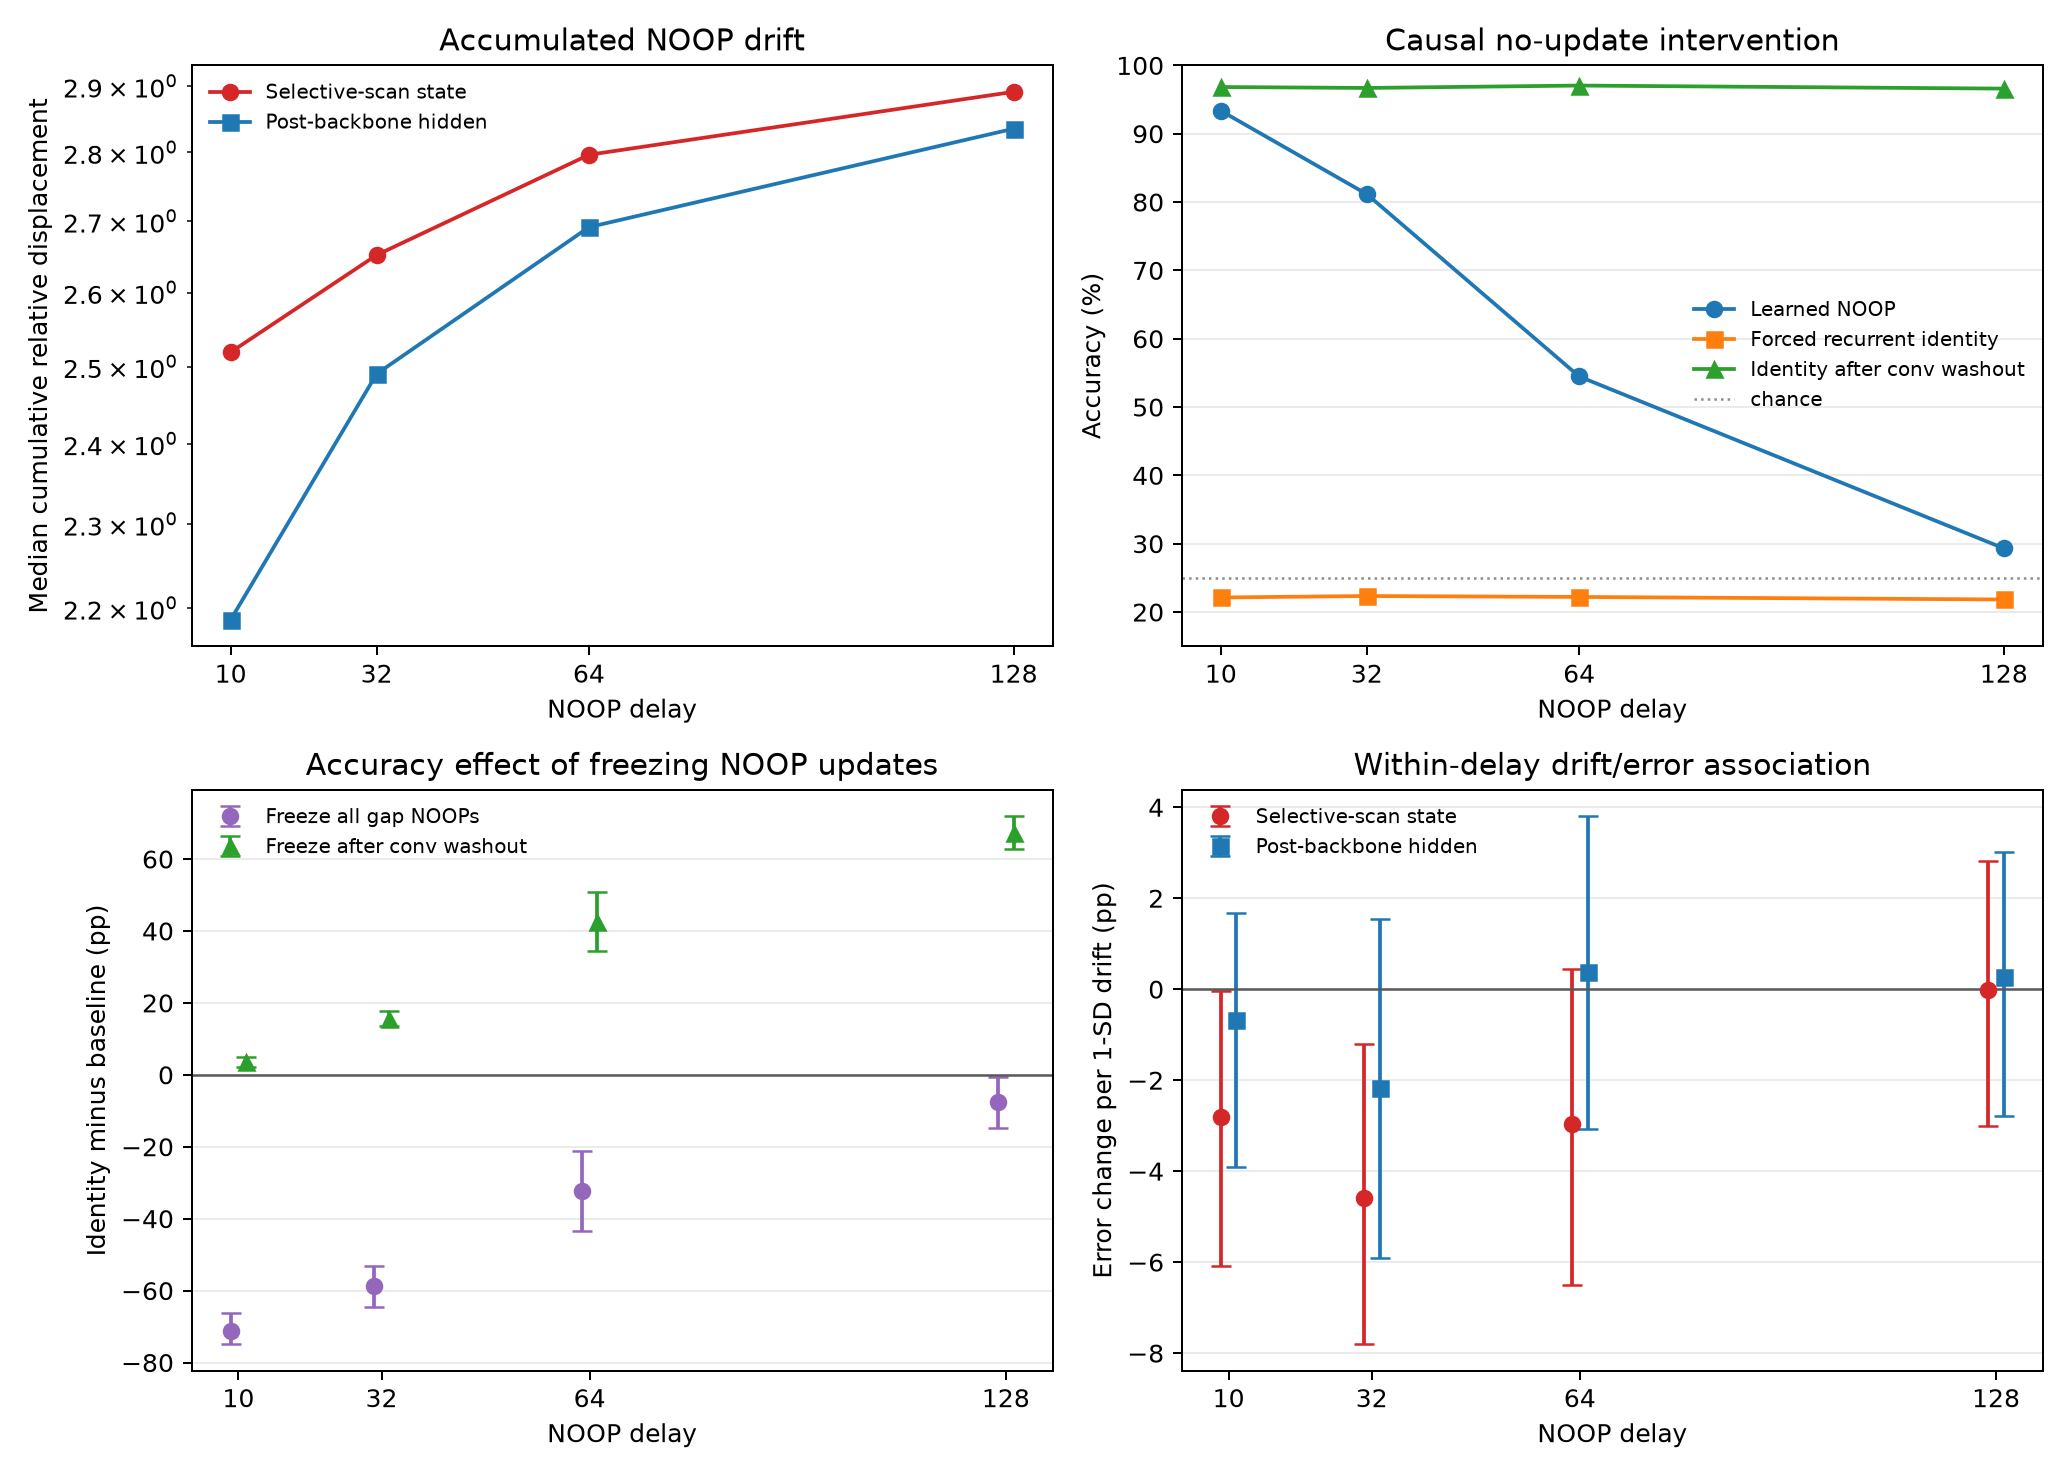
\includegraphics[width=0.82\linewidth]{figures/noop_identity_diagnostic.png}
\caption{NOOP identity diagnostic. Immediate freezing removes necessary convolutional settling (orange/purple), while freezing only after three washout steps preserves near-97\% retrieval (green). Raw drift alone is not sufficient evidence; the controlled intervention is the discriminating result.}
\label{fig:h4}
\end{figure}

\subsection{H5: retention versus readout accessibility}
The H4 rescue motivates a finer question: if attenuation is reduced, does the original classifier use the preserved information? We multiply recurrent decay during the 511-step NOOP interval by \(\alpha\), where \(\alpha=1\) is the trained dynamics, \(\alpha=0.1\) slows attenuation, and \(\alpha=0\) removes it while leaving the input-write and output pathways active. The backbone is frozen. Independent five-class linear probes are trained on disjoint long-horizon training sequences and evaluated on a held-out set at three internal locations:
\begin{itemize}
\item P1 receives the flattened \(64\times8\) recurrent state plus an 8D queried-key one-hot, because the state simultaneously contains all keys;
\item P2 receives the 64D SSM contraction \(C_th_t\), which tests what the learned query-conditioned state readout exposes;
\item P3 receives the final normalized 32D backbone feature; P4 is the original jointly trained \(\mathrm{Linear}(32,5)\) task head on that same feature.
\end{itemize}
P2 and P3 need no explicit key vector because they are sampled at the QUERY timestep, after the current query has conditioned convolution, \(C_t\), gating, and projection. Probes are trained separately so they diagnose accessibility at each location without changing the backbone or one another.

\begin{table}[!htbp]
\centering\small
\caption{H5 readout localization on a 511-step gap (accuracy in \%).}
\begin{tabular}{lrrrr}
\toprule
Decay multiplier & State + key probe & \(C_th_t\) probe & Final-feature probe & Original head \\
\midrule
\(\alpha=0\) & 86.3 & 67.6 & \cellcolor{softgreen}\textbf{99.6} & \cellcolor{softred}25.8 \\
\(\alpha=0.1\) & 59.8 & 48.4 & \cellcolor{softgreen}\textbf{97.7} & 29.3 \\
\(\alpha=1\) & 40.6 & 36.7 & 39.5 & \cellcolor{softred}25.0 \\
\bottomrule
\end{tabular}
\end{table}
At reduced decay, P3 is almost perfectly linearly separable while the original head remains near chance. Because both consume the same 32D feature, the difference is a decision-boundary mismatch, not missing classifier capacity. A fresh head trained only on ordinary length-32--128 frozen features also remains near chance at 511 steps, ruling out initialization or separate optimization as the explanation. Under natural decay, however, even P3 reaches only 39.5\%; readout retraining alone cannot repair information that the recurrence no longer exposes. H5 is therefore supported conditionally under altered retention, while natural long-horizon failure remains primarily a retention problem.
\begin{figure}[!htbp]
\centering
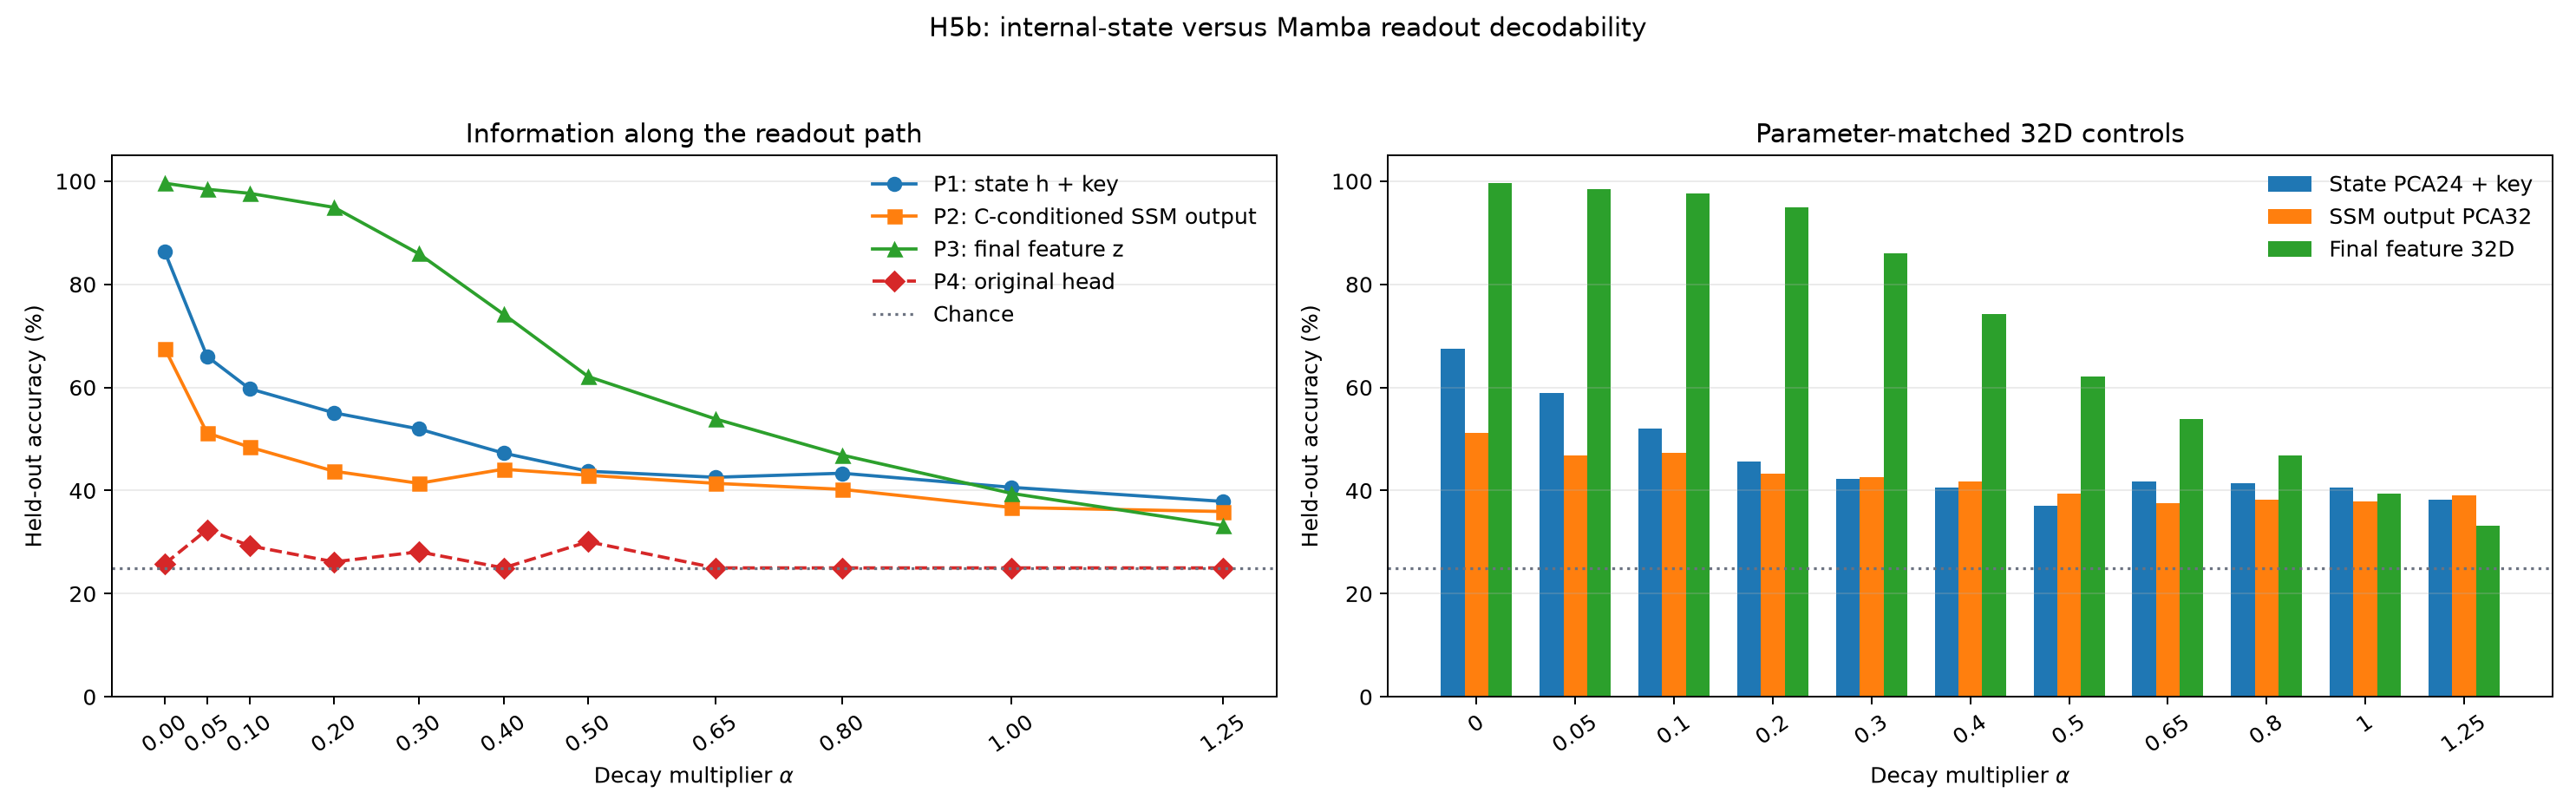
\includegraphics[width=0.95\linewidth]{figures/readout_decodability.png}
\caption{Held-out probe accuracy along the readout path versus decay multiplier. Under reduced decay, the final feature is highly decodable by a matched long-horizon probe while the original head remains near chance; under natural decay (\(\alpha=1\)), accessibility is much lower throughout.}
\label{fig:h5}
\end{figure}

\section{Supplementary Adaptive-Kernel Diagnostic}
The convolution-aware H4 result shows that local processing and recurrent retention interact: the first three apparent NOOPs still carry the width-four response to a preceding SET. We therefore ask whether the model benefits from choosing its effective local history by event context. This experiment is supplementary and deliberately separate from the Part B routing claim.

The adaptive causal kernel uses one width-eight depthwise kernel and mixes nested causal masks for effective widths \(\{1,2,4,8\}\). The adaptive router predicts mixture weights from the current token-side representation; the parameter-matched static ablation learns one sequence-independent mixture using the same kernel and parameter budget. A fixed-width-eight model separates the effect of receptive-field size from mixture learning. All models retain the original Mamba recurrence with \emph{no event-conditioned retention gate} and are trained from scratch for 1,500 updates on lengths 32--128. Because the router does not observe recurrent state directly, this test concerns token-conditioned local context, not explicit detection of whether a stored association is obsolete.

\addtocounter{table}{1}% preserve numbering of the full H5-controls table in the detailed record
\begin{table}[!htbp]
\centering\small
\caption{Adaptive-kernel architecture controls and assignment-defined stress results (seed 42, accuracy in \%).}
\resizebox{\linewidth}{!}{%
\begin{tabular}{lrrrrrr}
\toprule
Model & Params & ID-128 & OOD-512 & Gap-512 & Overwrite-512 & Final-gap probe \\
\midrule
Original Mamba (width 4) & 10,149 & 75.05 & 69.64 & 69.59 & 69.67 & 22.8 \\
Fixed width 8 & 10,405 & 76.59 & 71.94 & 71.54 & 71.86 & 22.6 \\
Static mixture & 10,729 & 77.62 & 72.94 & 72.61 & 72.56 & 24.4 \\
Adaptive mixture & 10,729 & \cellcolor{softgreen}78.95 & \cellcolor{softgreen}73.91 & \cellcolor{softgreen}73.58 & \cellcolor{softgreen}73.98 & 23.2 \\
\bottomrule
\end{tabular}
}
\end{table}

The distinction between the last three metrics is essential. OOD-512 uses ordinary random length-512 sequences. Gap-512 and Overwrite-512 use the assignment stress generators but still average over \emph{all} queries, most of which have short or moderate dependencies. Final-gap probe scores only the deliberately constructed last QUERY whose focus-key assignment spans approximately 511 steps. The adaptive model therefore improves aggregate stress accuracy without solving the extreme dependency: 73.58\% Gap-512 coexists with only 23.2\% on the final-gap probe.

\begin{figure}[!htbp]
\centering
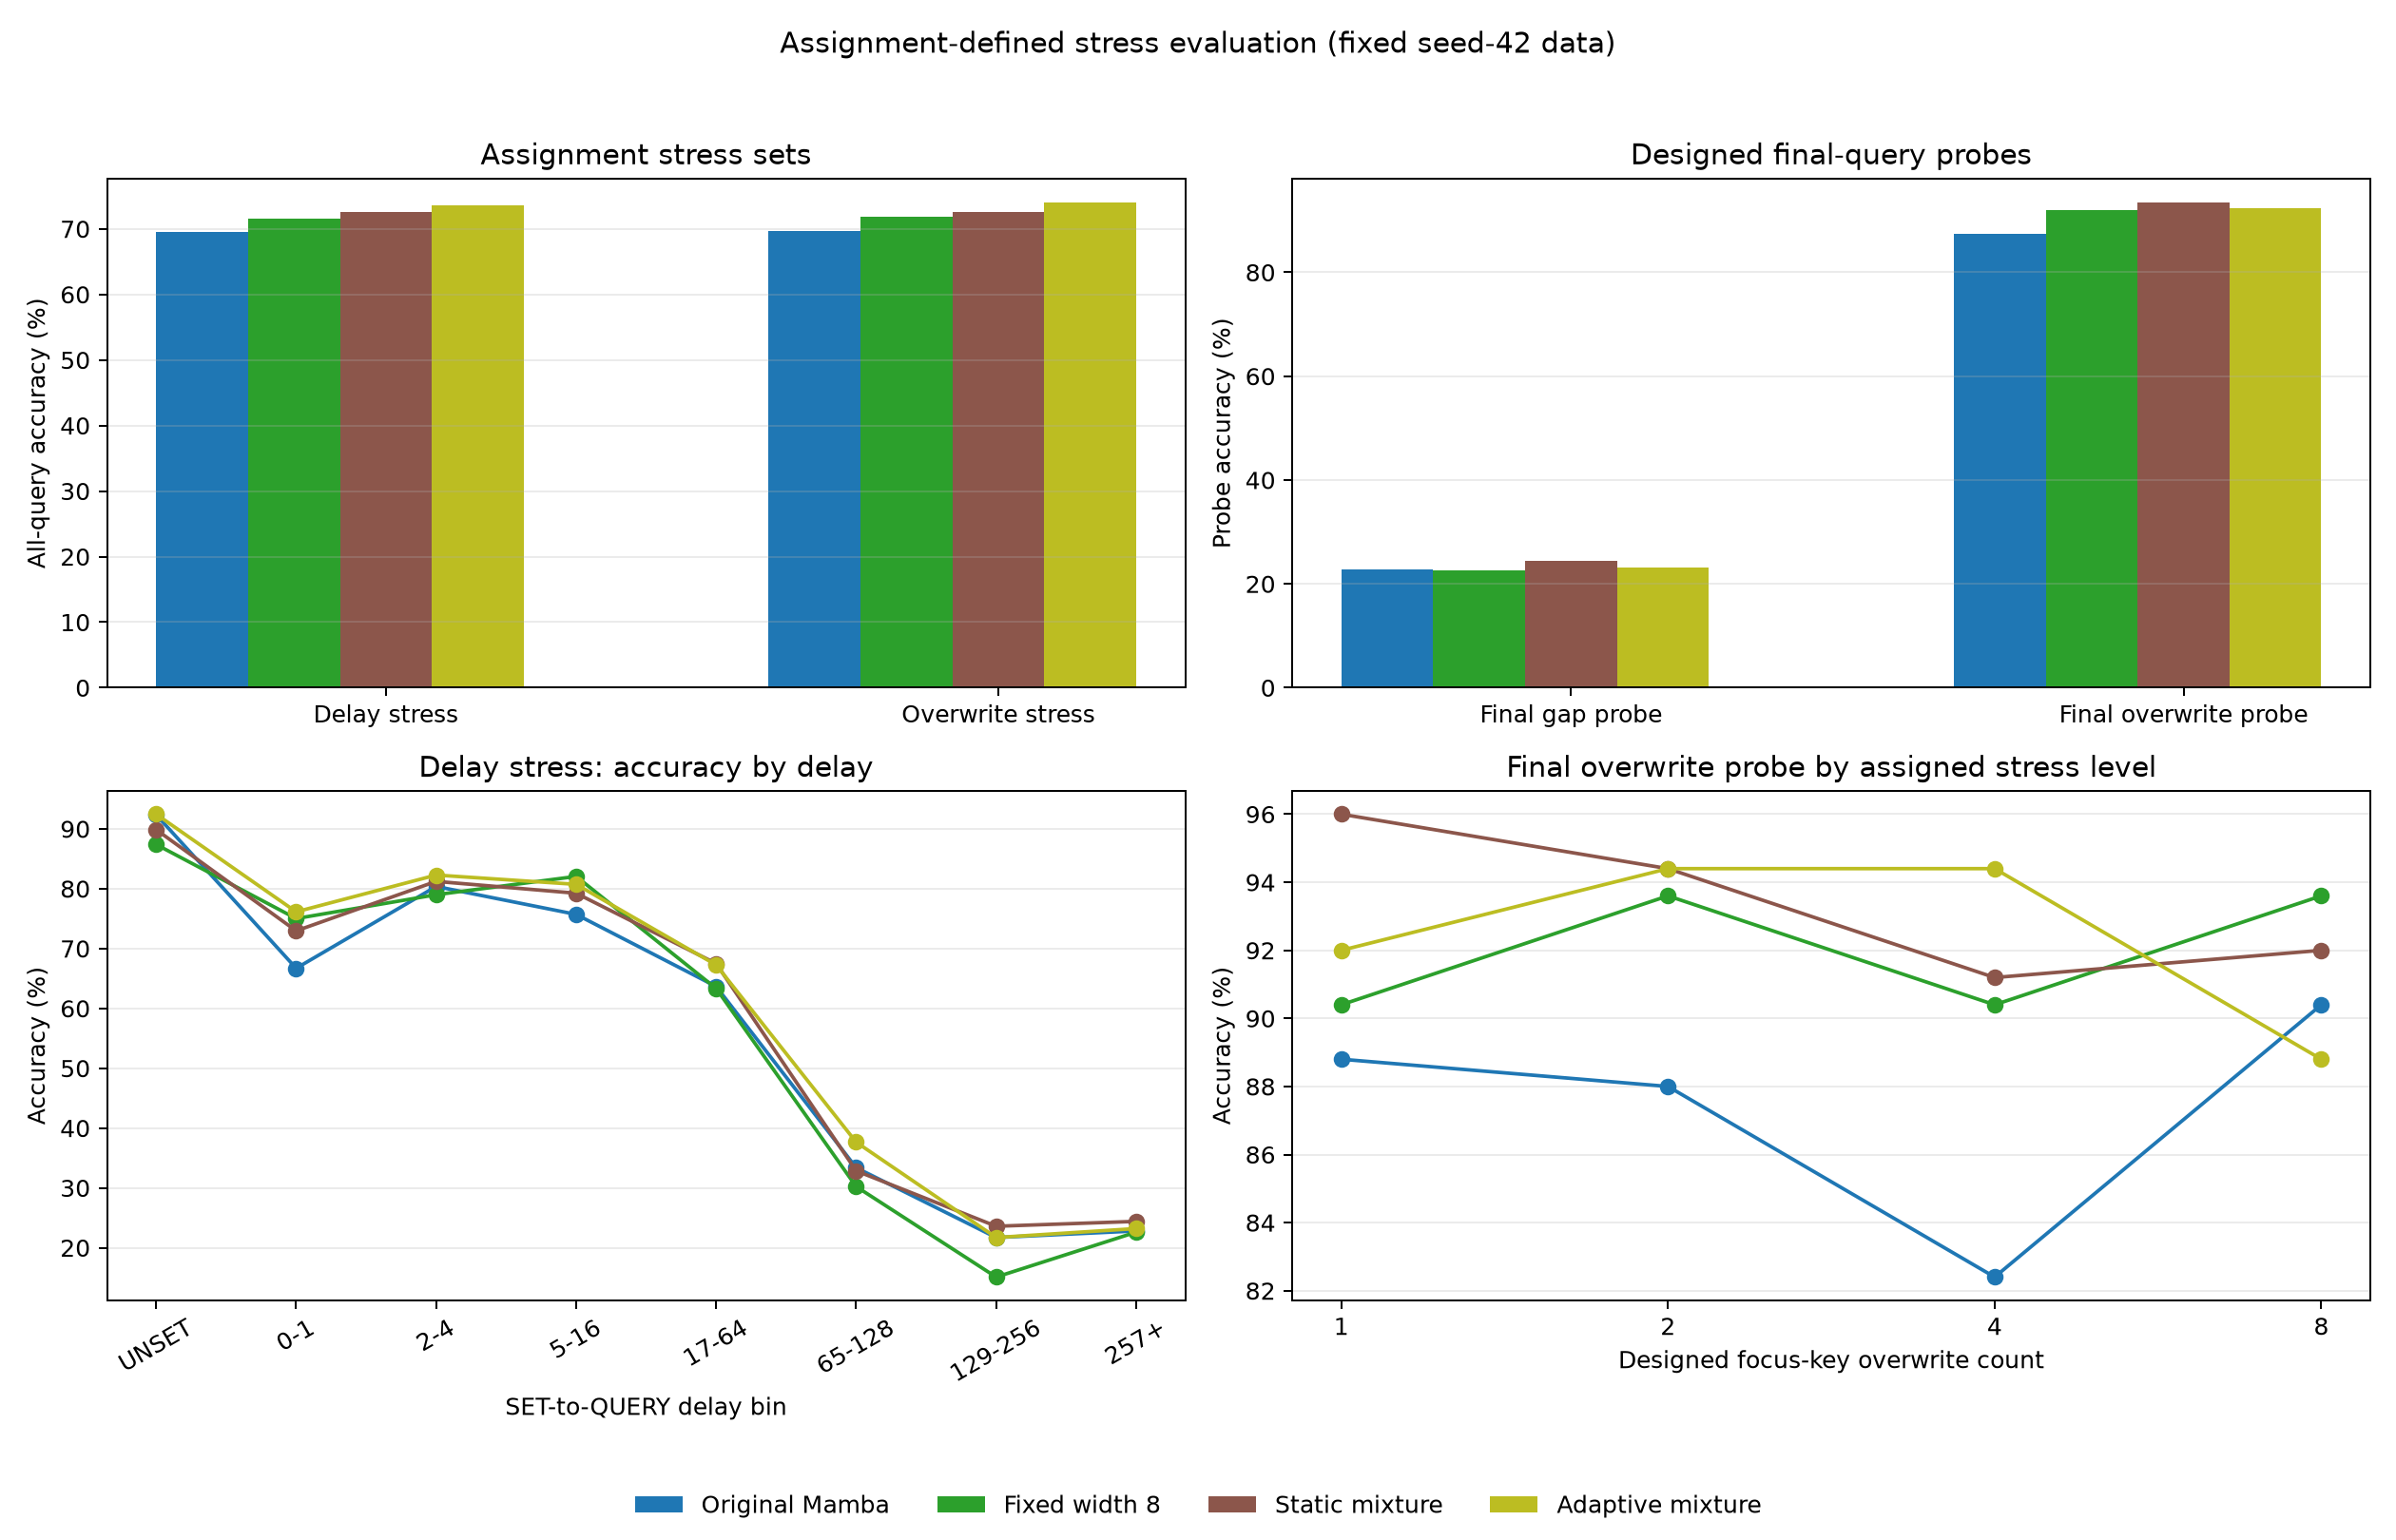
\includegraphics[width=0.98\linewidth]{figures/adaptive_assignment_stress.png}
\caption{Assignment-defined length-512 stress tests and controlled final-query probes for the original width-four model, fixed width eight, static mixture, and adaptive mixture. Aggregate stress accuracy improves with the larger-kernel variants, but every model remains near chance on the deliberately constructed final-gap query.}
\label{fig:adaptive-stress}
\end{figure}

\begin{table}[!htbp]
\centering\small
\caption{Controlled final-query probes and paired adaptive-kernel contrasts.}
\begin{tabularx}{\linewidth}{p{0.29\linewidth}rrrY}
\toprule
Contrast & Reference (\%) & Adaptive (\%) & Effect (pp) & 95\% paired CI / interpretation \\
\midrule
Final gap: adaptive vs static & 24.4 & 23.2 & -1.2 & $[-5.6,3.0]$; both near chance \\
Final overwrite: adaptive vs static & 93.4 & 92.4 & -1.0 & $[-3.2,1.2]$; no adaptive benefit \\
Final overwrite: adaptive vs original & 87.4 & 92.4 & +5.0 & $[1.2,8.8]$; capacity/local-mixing gain \\
\bottomrule
\end{tabularx}
\end{table}

The adaptive-versus-static rows are the mechanism test. Their paired intervals include zero on both controlled probes, and the point estimates favor static mixing. Adaptive exceeds original Mamba on final overwrite, but the static control shows that wider/local mixing capacity, rather than input-dependent selection, is the conservative explanation. The router itself selects expected widths 7.99, 6.16, and 7.55 for NOOP, SET, and QUERY events, so it does learn event dependence; that dependence simply does not yield the predicted controlled advantage.

\begin{figure}[!htbp]
\centering
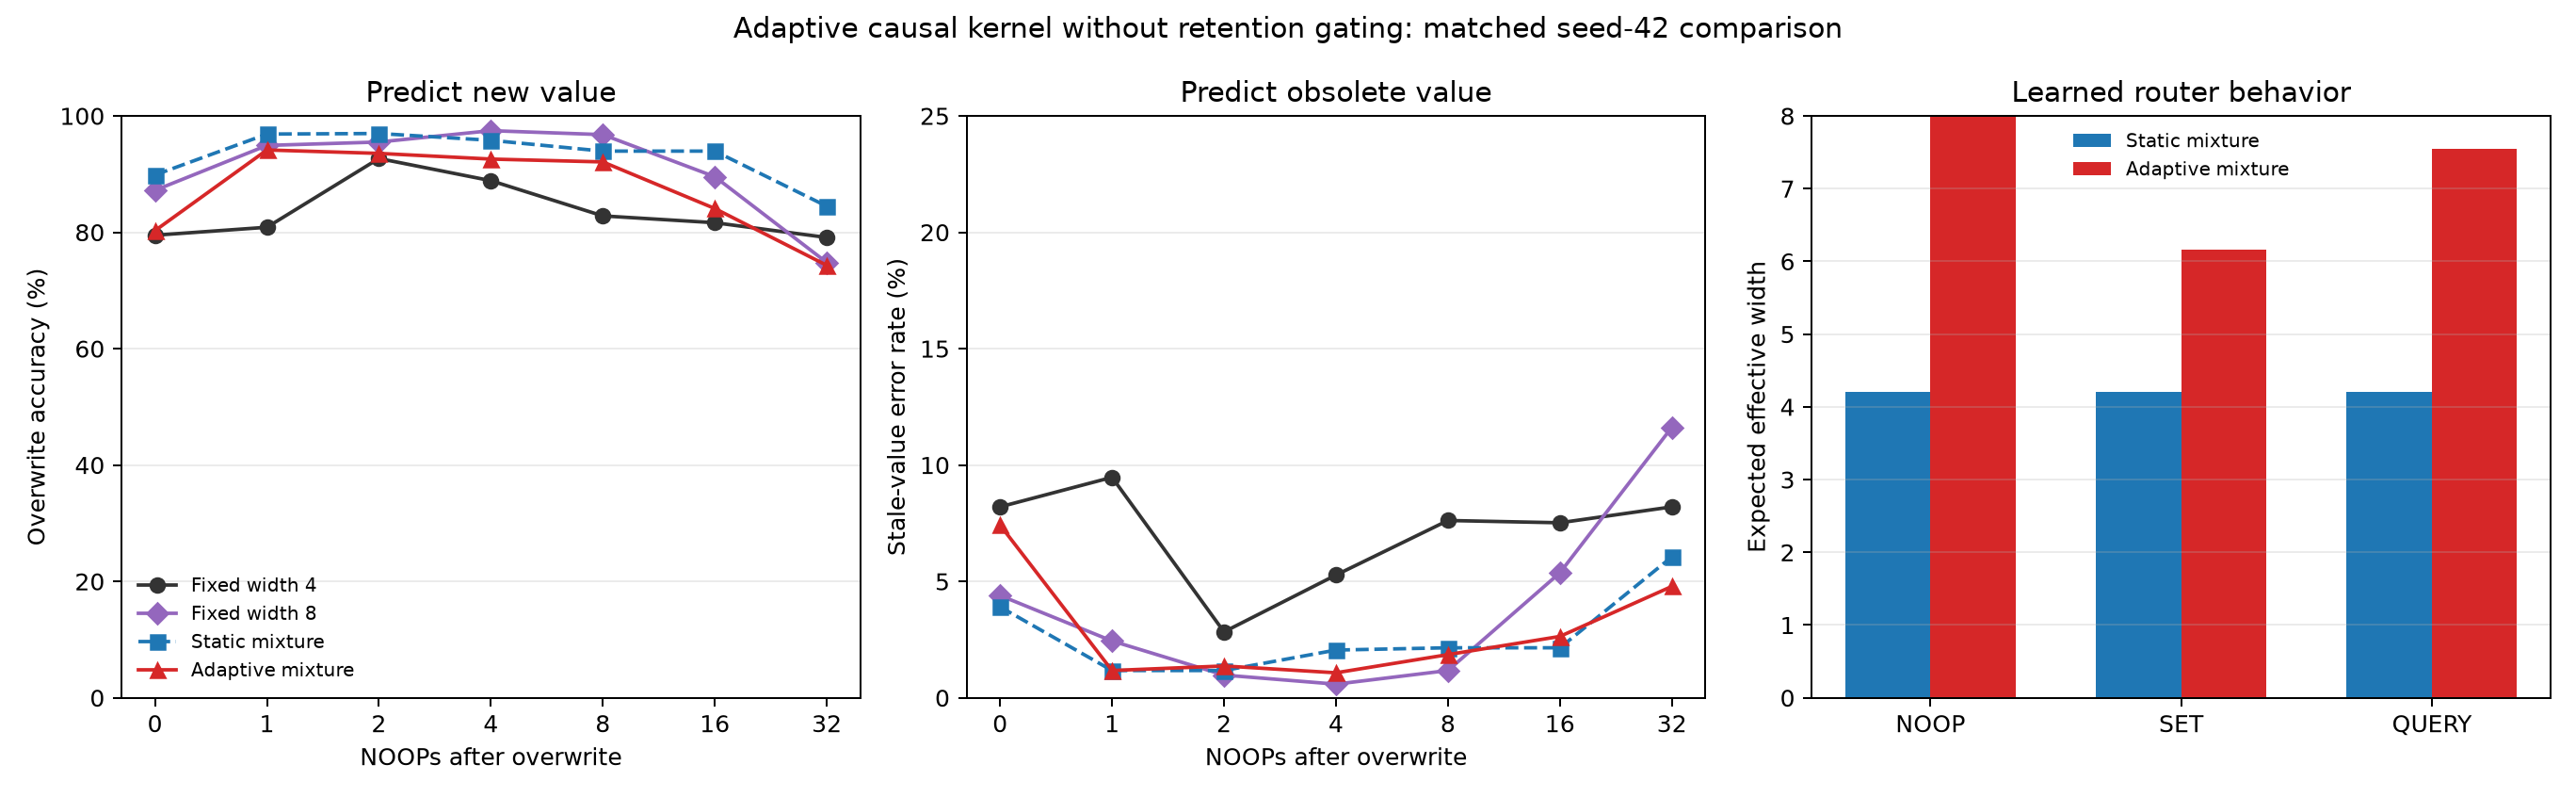
\includegraphics[width=0.98\linewidth]{figures/adaptive_kernel_comparison.png}
\caption{Direct static-versus-adaptive kernel diagnostic. The left and center panels measure correct-new-value accuracy and stale-value errors after an overwrite; the right panel confirms that the adaptive router selects event-dependent effective widths. Despite learning different widths for NOOP, SET, and QUERY, adaptive mixing does not consistently outperform the parameter-matched static mixture.}
\label{fig:adaptive-kernel}
\end{figure}

Training cost was measured for the complete 1,500-update runs on the same GTX 1650. Original Mamba, fixed width eight, static mixture, and adaptive mixture required 449.6, 524.2, 656.6, and 1,096.4 seconds, respectively. Recorded peak GPU allocations were 50.7, 50.7, 54.3, and 54.8 MiB. Adaptive mixing is therefore 2.44$\times$ slower than original and 1.67$\times$ slower than its parameter-matched static control, while adding only 0.5 MiB over that control; compute time, not memory, is the main engineering cost.

\begin{figure}[!htbp]
\centering
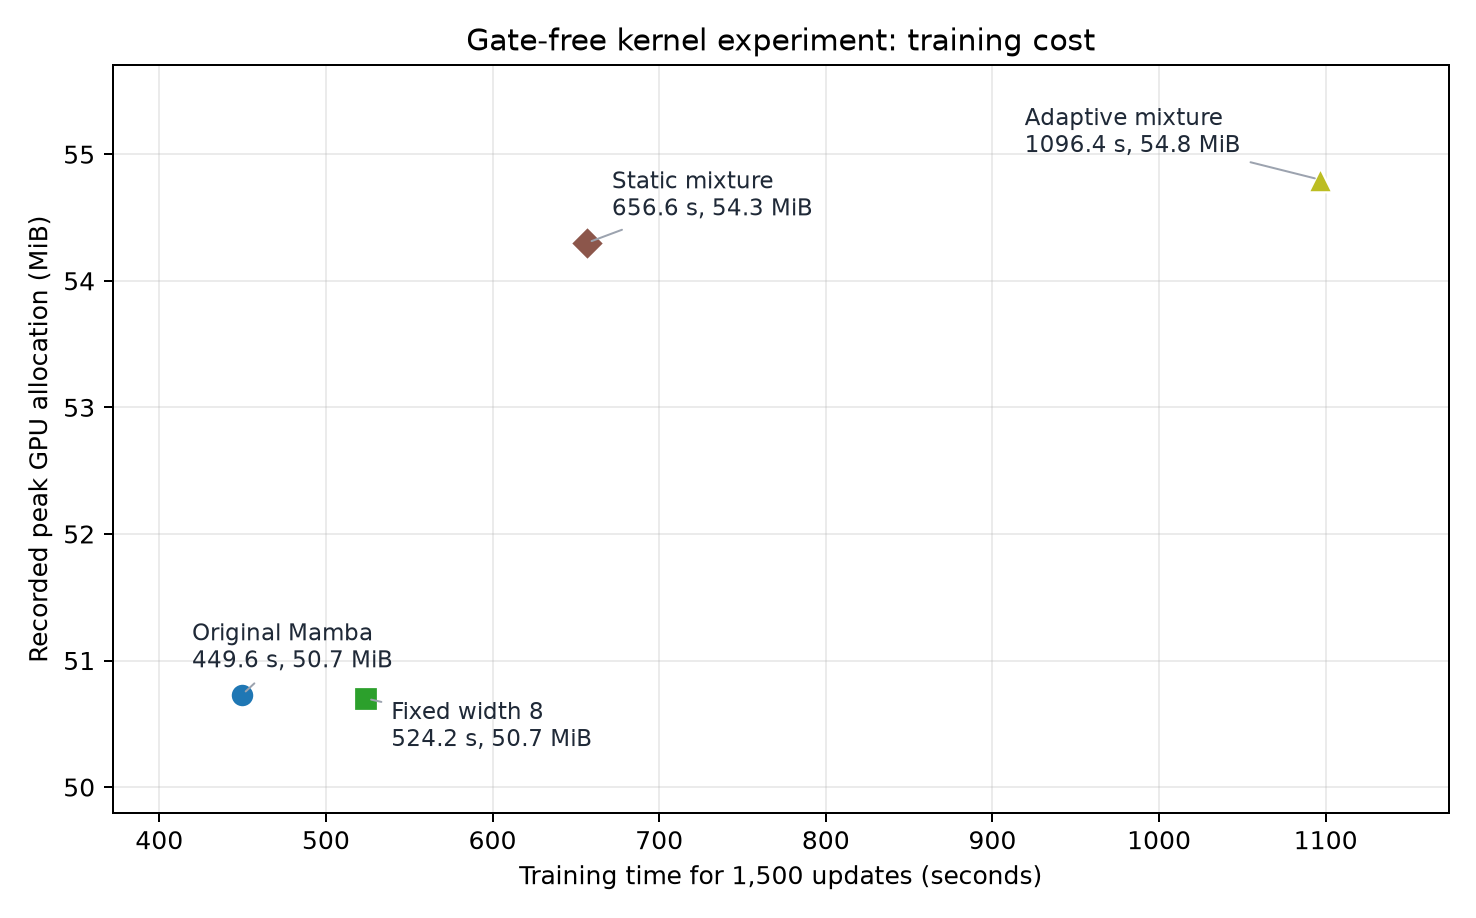
\includegraphics[width=0.82\linewidth]{figures/kernel_resource_tradeoff.png}
\caption{Measured training time and recorded peak GPU allocation for the gate-free kernel experiment. Adaptive mixing has only a modest memory premium over static mixing, but a substantial runtime premium.}
\label{fig:kernel-resources}
\end{figure}

\small\colorbox{softamber}{\parbox{0.93\linewidth}{\textbf{Supplementary verdict:} token-conditioned convolution is not supported over matched static mixing: adaptive is 1.2 pp worse on final gap and 1.0 pp worse on final overwrite, both intervals include zero, and extreme retention remains near chance.}}

\section{H7--H8: Trained Slow-Memory Recurrence}
\subsection{From timescale separation to identity-default memory}
The causal NOOP result motivates a trained rather than oracle-controlled transition. We partition the eight SSM modes into four fast and four slow modes. Fast rates are constrained above 1.0, while slow rates are constrained below 0.004; an initialization-only control removes the constraint after initialization. Frozen linear probes receive either the $64\times4$ fast state, the $64\times4$ slow state, or the complete $64\times8$ state, concatenated with the queried key. The constrained model concentrates more delay-511 information in the slow group and raises original-head accuracy from 25.0\% for original Mamba to 39.5\%. However, an H7b interpolation gate,
\[
h_t^S=(1-g_t)\odot h_{t-1}^S+g_t\odot \widetilde h_t^S,
\]
improves delay-511 accuracy to 62.1\% while sharply reducing immediate overwrite accuracy to 68.2\% and raising stale-value errors to 25.5\%. A single gate therefore entangles desirable retention with undesirable resistance to replacement.

\subsection{H8 architecture and decisive control}
H8 separates erasure of old slow memory from incorporation of the current write:
\begin{align}
h_t^F &= e^{\Delta_tA^F}\odot h_{t-1}^F+(\Delta_tB_tu_t)^F,\\
h_t^S &= (1-r_t)\odot h_{t-1}^S+w_t\odot(\Delta_tB_tu_t)^S.
\end{align}
After updating the fast state, a compact channel-wise router computes
\[
r_t=\sigma(f_r(u_t,q_t^F,e_t)),\qquad
w_t=\sigma(f_w(u_t,q_t^F,e_t)),
\]
where $q_t^F\in\mathbb R^{64}$ is a learned mode-weighted fast-state summary and $e_t$ is a learned 16-dimensional embedding of the current event token. Each 64-dimensional gate broadcasts over the four slow modes. The erase bias starts at $-4$ and the write bias at $-2$, favoring passive retention while preserving a usable write gradient.

The decisive tied control retains every router parameter and the same 13,605-parameter total, but uses
\[
r_t=w_t=\sigma\!\left(\tfrac12(f_r+f_w)\right).
\]
Thus independent H8 minus tied H8 isolates the effect of allowing different erase and write decisions; it is not confounded by capacity. Both models use the same seed-42 data order, AdamW settings, batch size, and 1,500 updates on lengths 32--128. Evaluation uses 256 balanced held-out examples per delay, independently trained fast/slow/full probes, and 192 balanced overwrite designs per pre/post-delay cell. Old and new values always differ when computing stale-value error rate (SVER).

\begin{table}[!htbp]
\centering\small
\caption{H8 primary results (seed 42, accuracy in \%). Long probes are diagnostic and use separate long-horizon supervision.}
\resizebox{\linewidth}{!}{%
\begin{tabular}{lrrrrrrrr}
\toprule
Model & Params & Validation & Delay-511 head & Slow short probe & Slow long probe & Immediate overwrite & Post-32 overwrite & Post-32 SVER \\
\midrule
Constrained fast/slow M1a & 10,149 & 82.23 & 39.45 & 31.64 & 57.81 & 97.40 & 73.44 & 26.04 \\
H8 independent $r,w$ & 13,605 & 95.18 & 31.25 & 29.69 & 39.84 & 100.00 & 91.15 & 3.12 \\
H8 tied $r=w$ & 13,605 & \cellcolor{softgreen}99.63 & \cellcolor{softgreen}40.23 & 28.12 & 52.73 & 100.00 & \cellcolor{softgreen}100.00 & \cellcolor{softgreen}0.00 \\
\bottomrule
\end{tabular}}
\label{tab:h8-primary}
\end{table}

Independent H8 is 8.20 points worse than M1a at delay 511 (paired 95\% bootstrap CI ([-16.41,-0.39])) and 8.98 points worse than the tied control (CI ([-16.80,-1.56]), (n=256)). The interval for the decisive independent-versus-tied comparison excludes zero in the direction opposite to H8's prediction. Figure~\ref{fig:h8-retention} shows that independent gating begins degrading by delay 32, whereas tied gating is perfect through delay 64 and remains competitive with M1a at 511.

\begin{figure}[!htbp]
\centering
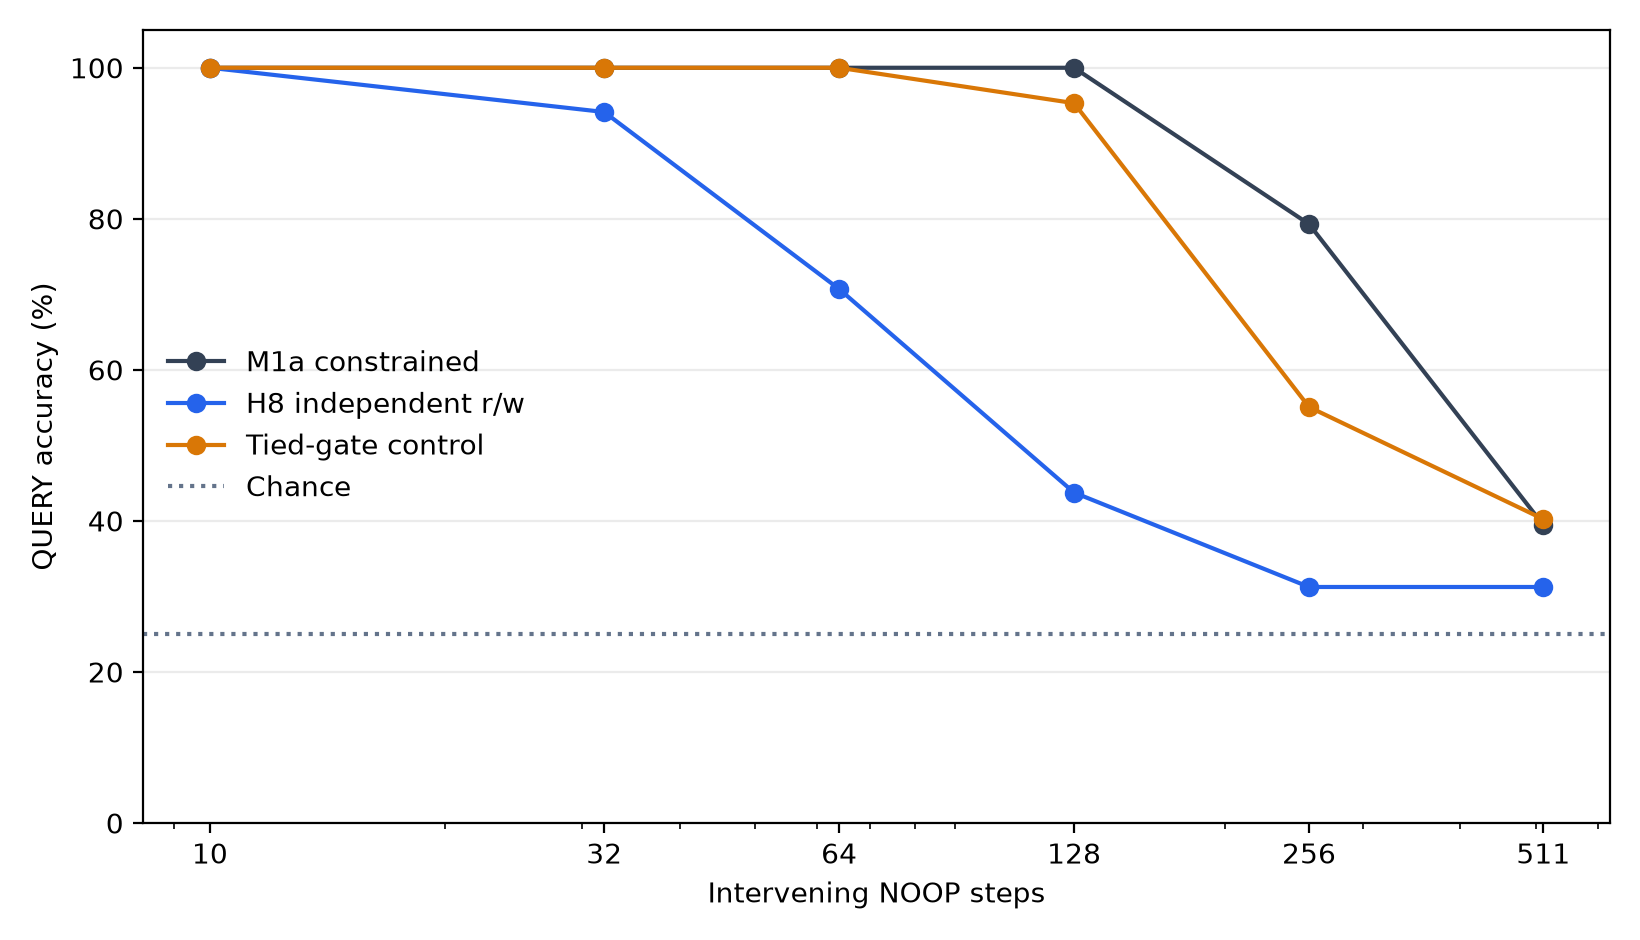
\includegraphics[width=0.82\linewidth]{figures/h8_retention_accuracy.png}
\caption{Original short-trained head on balanced retention probes. Independent erase/write gating underperforms both the constrained fast/slow precursor and the parameter-matched tied control at long delays. Chance is 25\%.}
\label{fig:h8-retention}
\end{figure}

\subsection{Why independent gates fail}
The gate audit in Figure~\ref{fig:h8-gates} provides a mechanistic explanation. Independent H8 learns larger writes for SET than NOOP (14.5\% versus 8.3\%), but its erase gate is paradoxically larger on NOOP than on SET (5.6\% versus 3.9\%). It therefore continues removing old slow memory during logically passive events. The tied control instead learns a clean event-selective policy: approximately 1.8\% on NOOP, 8.4\% on SET, and 2.5\% on QUERY. Its cumulative relative slow-state drift at delay 511 is 1.480, versus 3.494 for independent H8 and 2.793 for M1a.

\begin{figure}[!htbp]
\centering
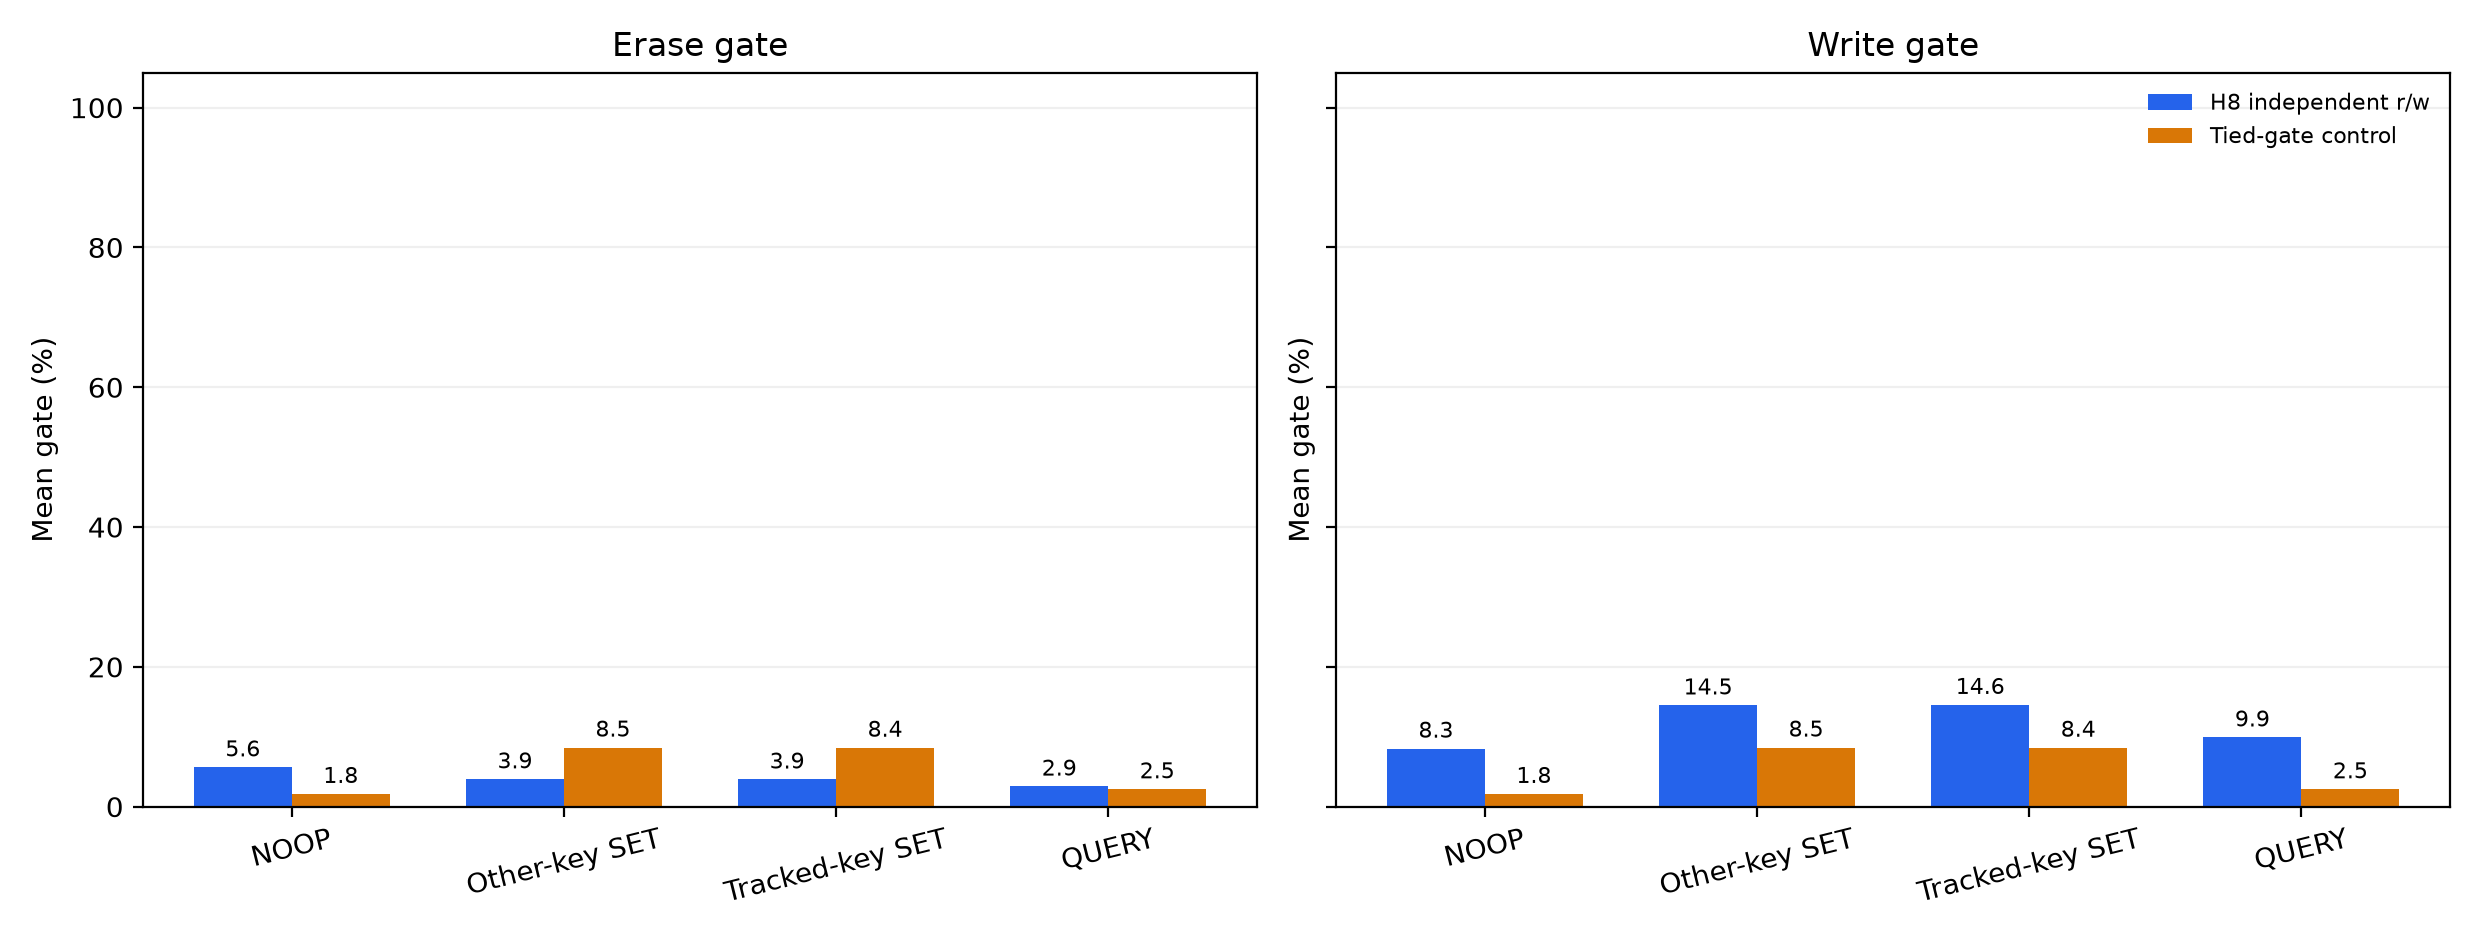
\includegraphics[width=0.94\linewidth]{figures/h8_event_gates.png}
\caption{Mean learned slow-memory gates by event category. The independent model separates writing from erasure, but erases more strongly on NOOP than SET. The tied control suppresses passive updates and opens primarily on SET events.}
\label{fig:h8-gates}
\end{figure}

The overwrite grid in Figure~\ref{fig:h8-overwrite} rules out the opposite failure mode. Tied gating preserves 100\% overwrite accuracy and 0\% SVER through 32 post-overwrite NOOPs while retaining 96.88\% of unmodified values. Independent H8 also improves replacement over M1a, but pure retention is only about 49\%, so its low SVER is not evidence of a solved memory system: it often loses the old value even when no overwrite occurs.

\begin{figure}[!htbp]
\centering
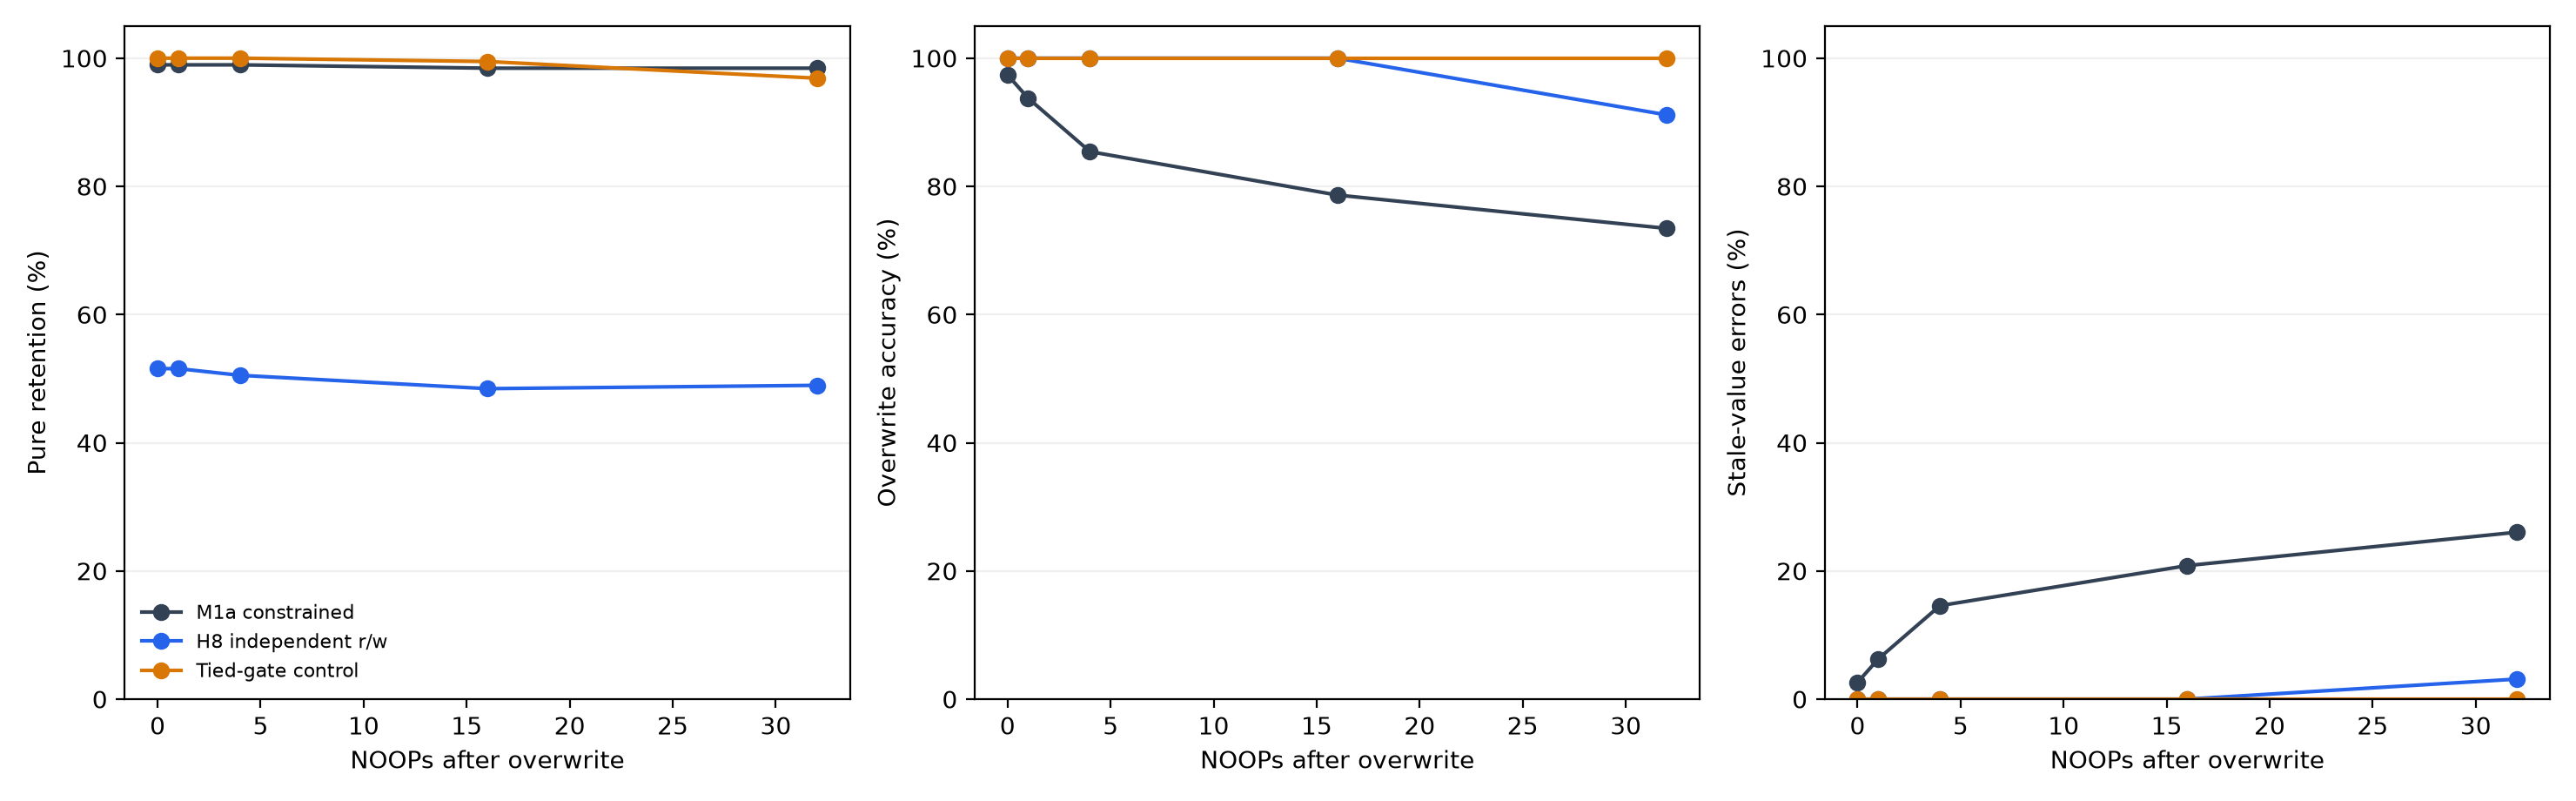
\includegraphics[width=0.98\linewidth]{figures/h8_overwrite_tradeoff.png}
\caption{Pre-delay 100 overwrite diagnostic. Left: pure retention without overwrite. Center: correctness after replacing the value. Right: predictions of the obsolete value. The tied control simultaneously preserves and replaces; independent H8 replaces well but fails pure retention.}
\label{fig:h8-overwrite}
\end{figure}

\small\colorbox{softred}{\parbox{0.93\linewidth}{\textbf{H8 verdict:} independent erase/write gating is falsified in the seed-42 pilot. The parameter-matched tied gate is both simpler in operation and better on validation, delay-511 retrieval, drift, overwrite accuracy, and stale-value errors. This is a one-seed architecture result and requires multi-seed confirmation.}}

\section{Failure Analysis, Limitations, and Next Step}
The experiments eliminate several attractive explanations. Aggregate length generalization is not long-horizon memory; suppressing writes does not repair interference; routed capacity does not imply key isolation; and adaptive local context does not solve a 511-step dependency. The evidence instead supports primary recurrent-retention failure plus secondary readout misalignment: passive transitions attenuate and reorganize state, and altered retention can move the final feature outside the short-trained decision geometry.
\begin{table}[!htbp]
\centering\small
\caption{Evidence-weighted failure map.}
\begin{tabularx}{\linewidth}{p{0.22\linewidth}Y Y p{0.14\linewidth}}
\toprule
Bottleneck & Strongest evidence & Boundary of claim & Priority \\
\midrule
Passive transition / retention & 67.3-pp rescue at delay 128 after conv-aware identity & Oracle frozen intervention & \cellcolor{softred}\textbf{Primary} \\
Event-selective slow update & Tied H8: 40.23\% at delay 511, 100\% post-32 overwrite, 0\% SVER & Seed-42 trained pilot & \cellcolor{softamber}Promising \\
Cross-key interference & SET distractors lose 14--50 pp vs NOOP & Write suppression/routing does not solve it & \cellcolor{softamber}Secondary \\
Readout distribution shift & Same 32D feature: 99.6\% probe vs 25.8\% original head & Appears under modified decay; probe uses long labels & \cellcolor{softamber}Conditional \\
Key-specific write overlap & Keyed and tied routing differ by $<1$ pp & One architecture seed & \cellcolor{softgreen}Not supported \\
Adaptive local mixing & 23.2\% final-gap probe; -1.2 pp vs static & One seed; CI includes zero & \cellcolor{softgreen}Not primary \\
Independent erase/write & -9.0 pp vs tied H8 at delay 511 & One seed; paired CI excludes zero & \cellcolor{softgreen}Not supported \\
\bottomrule
\end{tabularx}
\end{table}

Evidence is strongest for the paired convolution-aware identity rescue and weaker for single-seed architectures or probes trained with long-horizon labels. We therefore treat sub-point gains as null, call probes decodability diagnostics, and do not present frozen interventions as deployable models. H8 supplies the trained pilot that the earlier diagnosis called for, but reverses the architectural expectation: the tied event-selective gate is better than independent erase/write gates. The prioritized follow-up is therefore a five-seed confirmation of tied H8 against M1a and H7b, with delay-511 accuracy, pure retention, overwrite accuracy, SVER, and drift declared jointly. A second ablation should remove event identity while retaining router capacity to test whether event selectivity, rather than merely slower dynamics, causes the gain.

\section{Conclusion}
The compact Mamba generalizes well in aggregate to length 512 but cannot reliably carry one assignment across hundreds of transitions. Passive retention reaches chance at delay 500; unrelated activity adds interference, yet write suppression and key routing do not remedy it; and convolution-aware identity nearly eliminates degradation through delay 128. Passive recurrent evolution is therefore the best-supported primary bottleneck. H8 converts this diagnosis into a trained recurrence, but the proposed independent erase/write mechanism is rejected: it produces more passive drift and significantly worse delay-511 accuracy than its parameter-matched tied control. The tied gate is the most promising trained pilot because it suppresses NOOP updates while retaining perfect overwrite behavior. The conservative conclusion is not that H8 solves long memory---40.23\% at delay 511 remains modest---but that event-selective near-identity transitions deserve multi-seed testing, whereas extra routing freedom and local-kernel capacity do not.

\section{Reproducibility and Attribution}
Fixed splits, checkpoints, predictions, intervals, and plots are under \texttt{results/}. Primary reproduction runs \texttt{train.py} with \path{configs/baseline.yaml}, \path{configs/proposed.yaml}, or \path{configs/ablation.yaml}, then \texttt{part\_b\_compare.py}. H8 uses \path{configs/h8_decoupled_event_gate.yaml} and \path{configs/h8_decoupled_tied_gate.yaml}, followed by \texttt{h8\_decoupled\_retention.py}. The final suite contains 51 passing tests, including H8 causality, parameter matching, gate equality for the tied control, and exact trace/model agreement. The readable model derives from John Ma's MIT-licensed \texttt{mamba-minimal}; the assignment supplied the generator and sample data. AI assistance supported scaffolding, experiment scripts, plotting, and editing. I selected the hypotheses and controls, executed and checked the experiments, and take responsibility for the conclusions.

\begin{thebibliography}{3}\small
\bibitem{s4} A. Gu, K. Goel, and C. R\'e. \emph{Efficiently Modeling Long Sequences with Structured State Spaces}. arXiv:2111.00396, 2021.
\bibitem{mamba} A. Gu and T. Dao. \emph{Mamba: Linear-Time Sequence Modeling with Selective State Spaces}. arXiv:2312.00752, 2023.
\bibitem{minimal} J. Ma. \emph{mamba-minimal}: a readable PyTorch implementation. \url{https://github.com/johnma2006/mamba-minimal}, MIT License.
\end{thebibliography}

\end{document}
